\documentclass[border=10pt]{standalone}
\usepackage{underscore}
\usepackage{tikz}
\usetikzlibrary{shapes,arrows,positioning,calc,backgrounds,matrix,fit,decorations.pathreplacing}

\newcount\index
\newcommand{\diaName}{default name}
\newcommand{\diaWidth}{10em}
\newcommand{\diaHeight}{2em}
\newcommand{\updateIndex}{\advance\index by 1\relax}
\newcommand{\lastId}{\diaName-\the\numexpr\index-1\relax}
\newcommand{\id}{\diaName-\the\index}

\newcommand{\record}[2]{
    \node[fixed node={\diaWidth}{\diaHeight},below=of \lastId,#1](\id){#2};
    \updateIndex
}
%%% environment struct
\newenvironment{struct}[3]
{
    \index=0
    \renewcommand{\diaName}{#1}
    \renewcommand{\diaWidth}{#2}
    \renewcommand{\diaHeight}{#3}
}
{
    \node[fit=(\diaName-0)(\lastId),inner sep=0pt](\diaName){};
}
%%% environment struct end


\tikzset{
    table/.style 2 args={
        draw,
        rectangle,
        inner sep=0pt,
        matrix of nodes,
        nodes in empty cells,
        nodes={
            draw,
            font=\ttfamily,
            align=center,
            text width=#1,
            outer sep=0pt,
            inner sep=0.3em,
            minimum height=1.6em
        },
        label={[align=center]90:\bf{#2}}
    },
    table/.default={10cm}{},
    right brace/.style 2 args={
        decorate,
        decoration={brace,amplitude=#1,raise=#2}
    },
    right brace/.default={8pt}{2pt},
    right note/.style={right=#1},
    right note/.default={0.3cm},
    left note/.style={left=#1},
    left note/.default={0.3cm},
    left brace/.style 2 args={
        decorate,
        decoration={brace,amplitude=#1,raise=#2,mirror}
    },
    left brace/.default={8pt}{2pt},
    right addr note/.style={right=#1},
    right addr note/.default={0.5cm},
    left addr note/.style={left=#1},
    left addr note/.default={0.5cm},
    arrow/.style={>=stealth',->},
    fixed node/.style 2 args={
        node distance=0,
        outer sep=0,
        inner sep=0,
        draw,
        font=\ttfamily,
        rectangle,
        minimum width=#1,
        minimum height=#2
    },
    title node/.style={rectangle,inner sep=1em},
    blank cell/.style={fill=white,minimum height=1cm},
    non blank cell/.style={fill=cyan!30,minimum height=#1}
}


\begin{document}
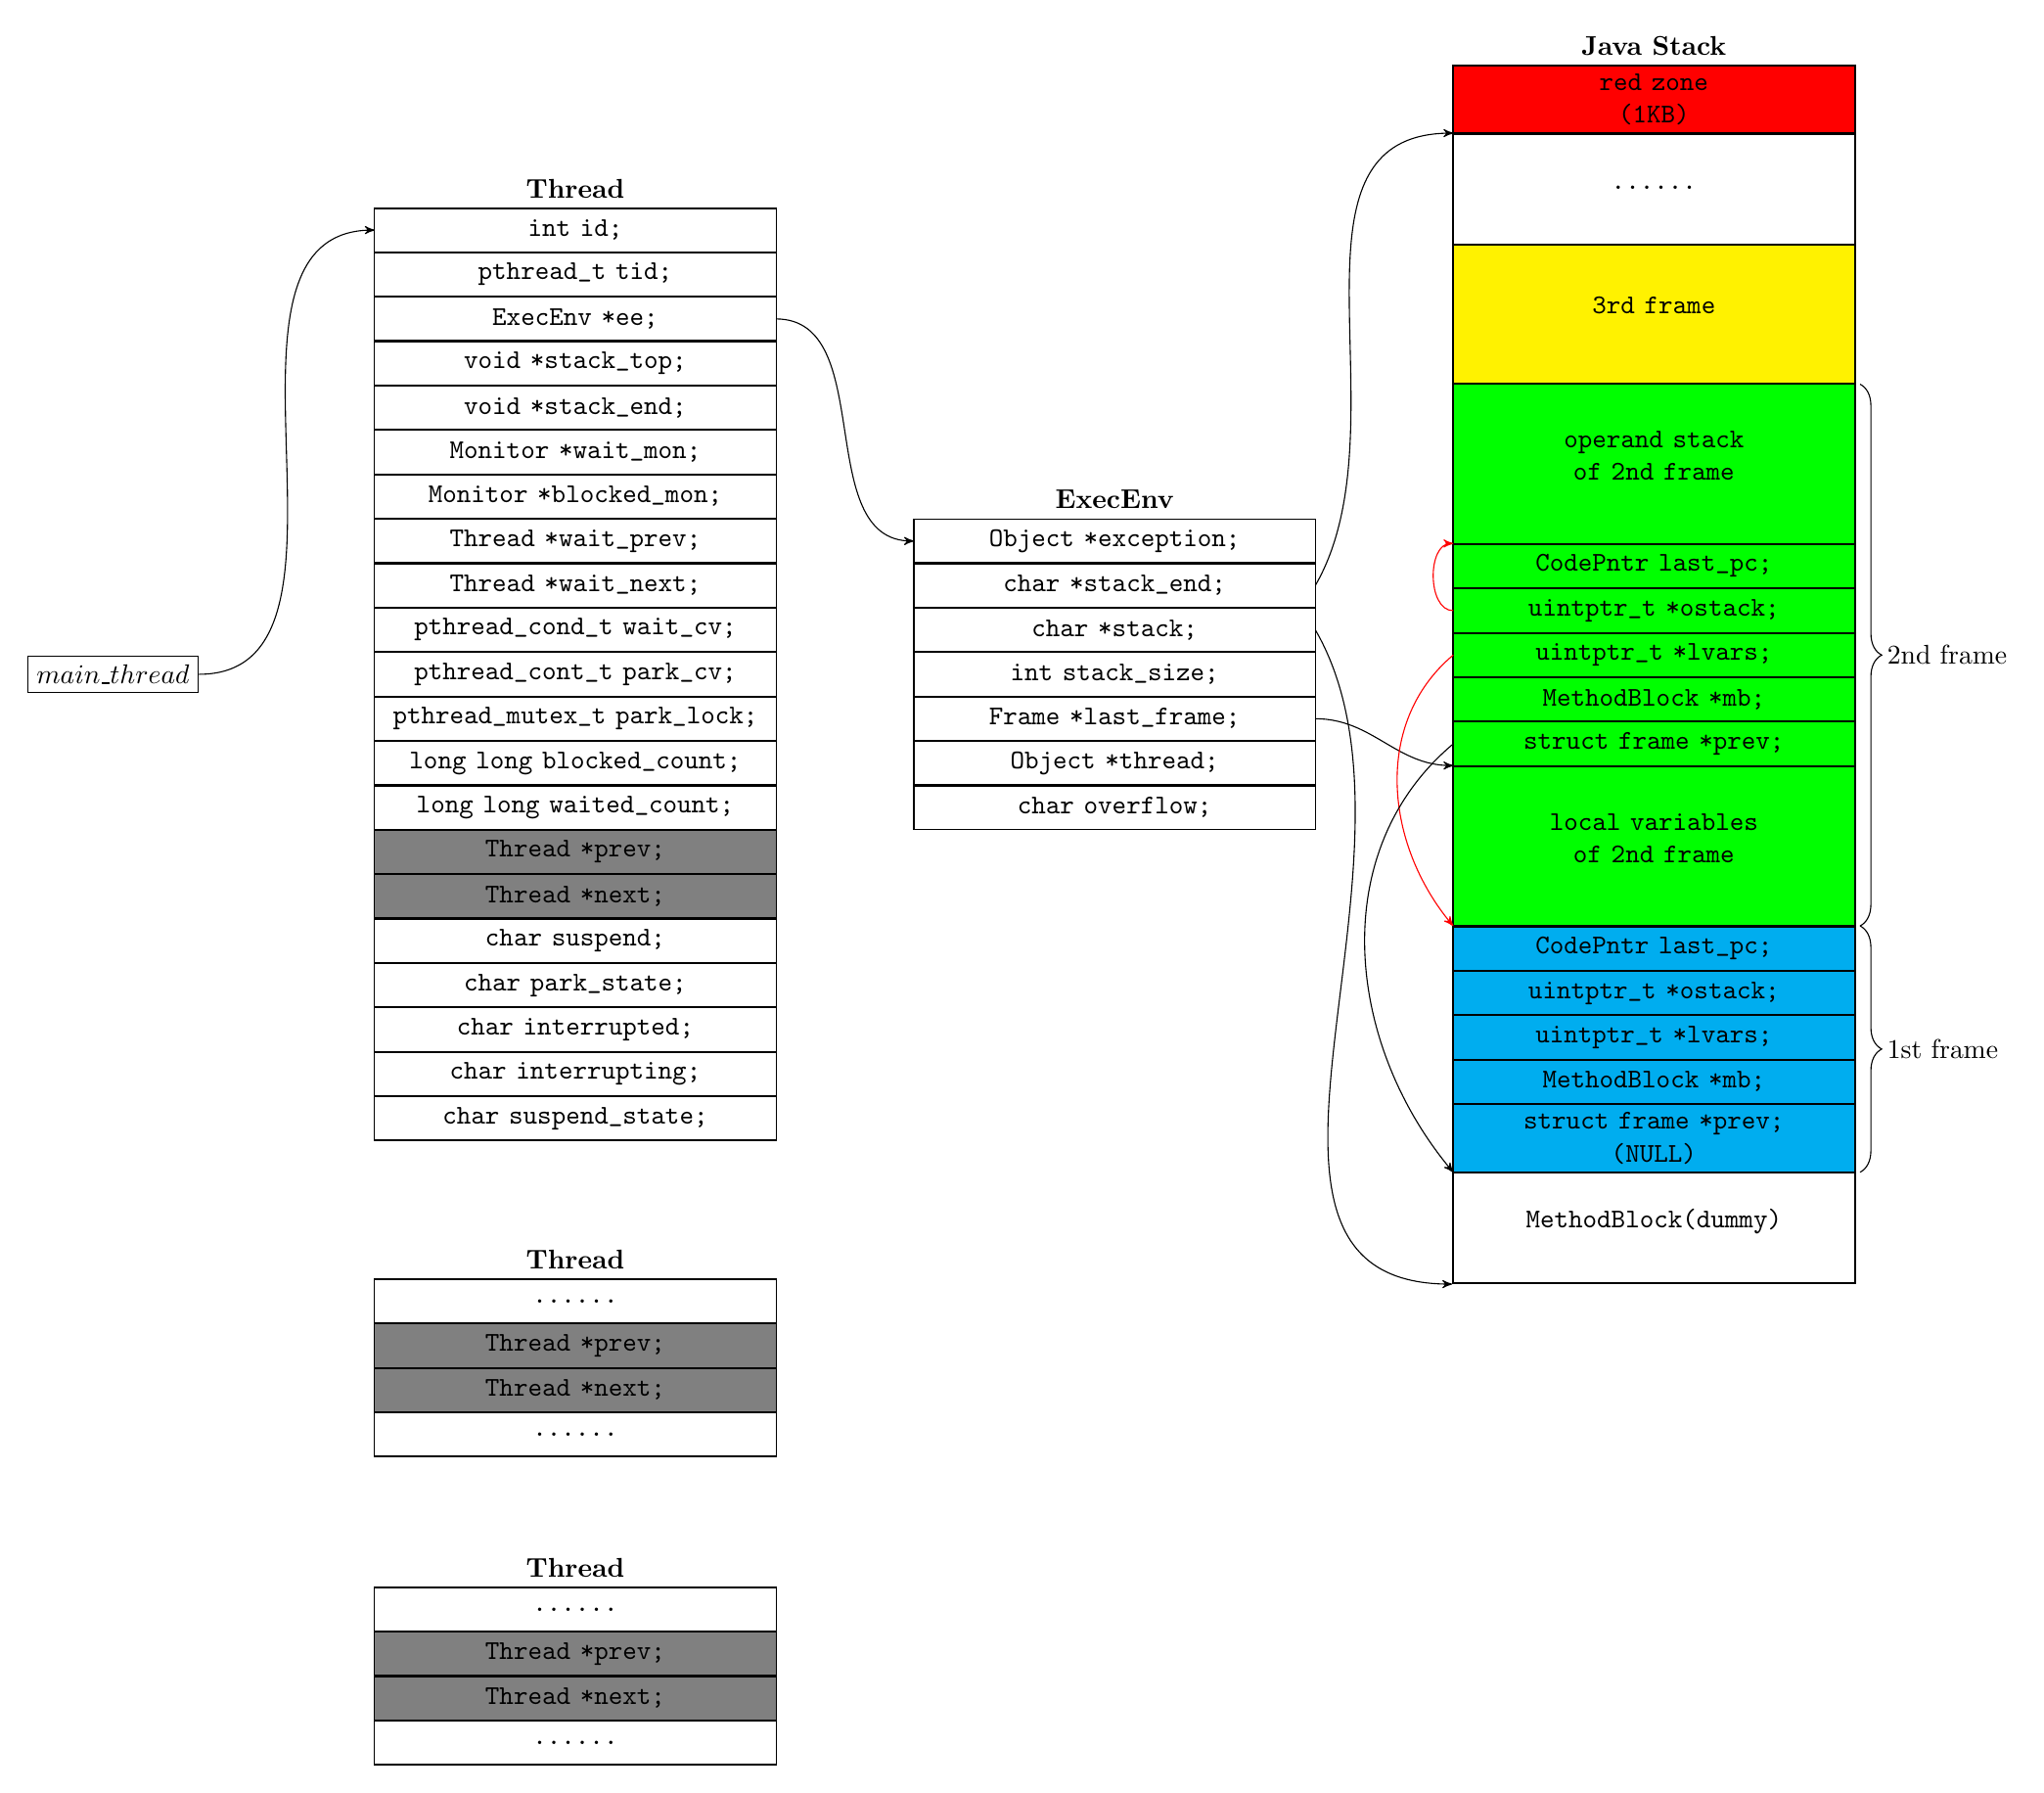
\begin{tikzpicture}

    %%% content
    \node (mainThread) [draw] {$main\textunderscore thread$};
    
    \matrix (thread) [table={5cm}{Thread}, right of=mainThread, xshift=5cm] {
        ||{int id;}\\
        ||{pthread_t tid;}\\
        |(ee)|{ExecEnv *ee;}\\
        ||{void *stack_top;}\\
        ||{void *stack_end;}\\
        ||{Monitor *wait_mon;}\\
        ||{Monitor *blocked_mon;}\\
        ||{Thread *wait_prev;}\\
        ||{Thread *wait_next;}\\
        ||{pthread_cond_t wait_cv;}\\
        ||{pthread_cont_t park_cv;}\\
        ||{pthread_mutex_t park_lock;}\\
        ||{long long blocked_count;}\\
        ||{long long waited_count;}\\
        |[fill=gray]|{Thread *prev;}\\
        |[fill=gray]|{Thread *next;}\\
        ||{char suspend;}\\
        ||{char park_state;}\\
        ||{char interrupted;}\\
        ||{char interrupting;}\\
        ||{char suspend_state;}\\
    };
    
    \matrix (thread2) [table={5cm}{Thread}, below of=thread, yshift=-8cm] {
        ||{......}\\
        |[fill=gray]|{Thread *prev;}\\
        |[fill=gray]|{Thread *next;}\\
        ||{......}\\
    };
    
    \matrix (thread3) [table={5cm}{Thread}, below of=thread2, yshift=-3cm] {
        ||{......}\\
        |[fill=gray]|{Thread *prev;}\\
        |[fill=gray]|{Thread *next;}\\
        ||{......}\\
    };
    
    \matrix (execEnv) [table={5cm}{ExecEnv}, right of=thread, xshift=6cm] {
        ||{Object *exception;}\\
        |(stack end)|{char *stack_end;}\\
        |(stack)|{char *stack;}\\
        ||{int stack_size;}\\
        |(last frame)|{Frame *last_frame;}\\
        ||{Object *thread;}\\
        ||{char overflow;}\\
    };
    
    \matrix (javaStack) [table={5cm}{Java Stack}, right of=execEnv, xshift=6cm] {
        |[fill=red](red zone)|{red zone\\(1KB)}\\
        ||{\\[.5em]......\\[.5em]\ }\\
        |[fill=yellow](third frame)|{\\[1em]3rd frame\\[1em]\ }\\
        |[fill=green](second ostack content)|{\\[.8em]operand stack\\ of 2nd frame\\[.8em]\ }\\
        |[fill=green]|{CodePntr last_pc;}\\
        |[fill=green](second ostack)|{uintptr_t *ostack;}\\
        |[fill=green](second lvars)|{uintptr_t *lvars;}\\
        |[fill=green]|{MethodBlock *mb;}\\
        |[fill=green](second prev)|{struct frame *prev;}\\
        |[fill=green](second lvars content)|{\\[.8em]local variables\\ of 2nd frame\\[.8em]\ }\\
        |[fill=cyan]|{CodePntr last_pc;}\\
        |[fill=cyan](first ostack)|{uintptr_t *ostack;}\\
        |[fill=cyan](first lvars)|{uintptr_t *lvars;}\\
        |[fill=cyan](first mb)|{MethodBlock *mb;}\\
        |[fill=cyan](first prev)|{struct frame *prev;\\(NULL)}\\
        ||{\\[.5em]MethodBlock(dummy)\\[.5em]\ }\\
    };
    
    %% lines
    \draw[arrow] (ee.east) to[out=0,in=180] (execEnv-1-1.west);
    \draw[arrow] (stack end.east) to[out=60,in=180] (red zone.south west);
    \draw[arrow] (stack.east) to[out=-60,in=180] (javaStack.south west);
    \draw[arrow] (last frame.east) to[out=0,in=180] (second prev.south west);
    \draw[arrow,draw=red] (second ostack.west) to[out=180,in=180] (second ostack content.south west);
    \draw[arrow,draw=red] (second lvars.west) to[out=220,in=130] (second lvars content.south west);
    \draw[arrow] (second prev.west) to[out=220,in=130] (first prev.south west);
    \draw[right brace] (second ostack content.north east) -- node[right note]{2nd frame} (second lvars content.south east);
    \draw[right brace] (second lvars content.south east) -- node[right note]{1st frame} (first prev.south east);
    \draw[arrow] (mainThread.east) to[out=0,in=180] (thread-1-1.west);
\end{tikzpicture}
\end{document}
